%!TEX encoding = UTF-8 Unicode

\section{Proposed Approach}

% BN can infer the actions just looking at the objects, effects, and verbal descriptions
% +
% HMM - inference of the action via the user movements
%Them open a subsection to explain the bayesian network, then another for the HMM and another for the fusion of the two.

In this paper, we combine (1)~the robot affordance model of~\cite{salvi:2012:smcb}, which associates verbal descriptions to the physical interactions of an agent with the environment, with (2)~the gesture recognition system of~\cite{saponaro:2013:crhri}, which infers the type of action from human user movements. Our main contribution is that of extending~\cite{salvi:2012:smcb} by relaxing the known-action assumption. We estimate the action performed by a human user during a \hr{} collaborative task, by employing statistical inference methods and \acp{HMM}. This provides two advantages. First, we can infer the executed action during training. Secondly, at testing time we can merge the action information obtained from gesture recognition with the information about affordances.

\begin{figure}
  \centering
  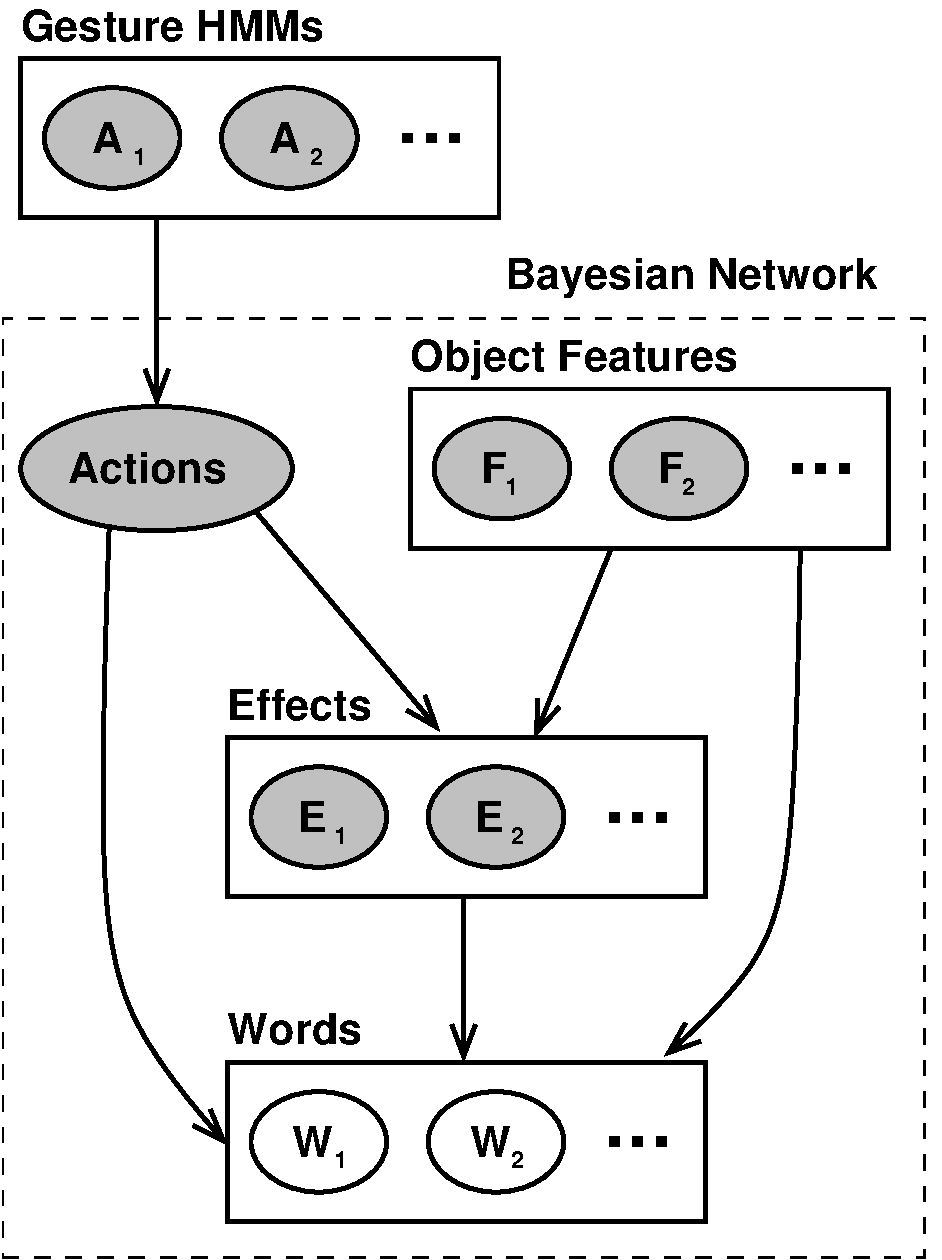
\includegraphics[width=0.8\columnwidth]{fullNetAbstract}
  \caption{Abstract representation of the probabilistic dependencies in the model. Shaded nodes are observable or measurable in the present study, and edges indicate Bayesian dependency.}
  \label{fig:model}
\end{figure}

\subsection{Affordance--Words \acl{BN}}
\label{sec:bn}

Following the method adopted in~\cite{salvi:2012:smcb}, we use a Bayesian probabilistic framework to allow a robot to ground the basic world behavior and verbal descriptions associated to it. The world behavior is defined by random variables describing: the actions~$A$, defined over the set~$\mathcal{A} = \{a_i\}$, object properties~$F$, over $\mathcal{F} = \{f_i\}$, and effects~$E$, over~$\mathcal{E} = \{e_i\}$. We denote~$X = \{A, F, E\}$ the state of the world as experienced by the robot. The verbal descriptions are denoted by the set of words~$W = \{w_i\}$. Consequently, the relationships between words and concepts are expressed by the joint probability distribution~$p(X,W)$ of actions, object features, effects, and words in the spoken utterance. The symbolic variables and their discrete values are listed in Table~\ref{tab:bnsymb}.

\begin{table}
    \centering
    \caption{Symbolic variables of the \acl{BN} from~\cite{salvi:2012:smcb} which we use in this work, with corresponding discrete values obtained from clustering. In addition, the full model also includes word variables~(see Fig.~\ref{fig:model}), whose values are the probabilities of the words occurring in the associated verbal description of an experiment - PUT THIS LAST PHRASE AS FOOTNOTE?.}
    \label{tab:bnsymb}
    \begin{tabular}{*{3}{l}} % left-aligned columns
    \toprule
    name   & description     & values \\
    \midrule
    Action & action          & grasp, tap, touch \\
    Shape  & object shape    & sphere, box \\
    Size   & object size     & small, medium, big \\
    ObjVel & object velocity & slow, medium, fast \\
    \bottomrule
    \end{tabular}
\end{table}

This joint probability distribution, that is illustrated by the part of Fig.~\ref{fig:model} enclosed in the dashed box, is estimated by the robot in an ego-centric way through interaction with the environment, as in~\cite{salvi:2012:smcb}. As a consequence, during learning, the robot knows what action it is performing with certainty, and the variable~$A$ assumes a deterministic value. This assumption is relaxed in the present study, by extending the model to the observation of external~(human) agents as explained below.

\subsection{Gesture \aclp{HMM}}

With regard to the gesture recognition \acsp{HMM}, we use the ones that we previously trained in~\cite{saponaro:2013:crhri} for spotting three manipulation-related gestures~(tapping, grasping, pushing). The \ac{HMM} for one gesture is defined by a set of (hidden) discrete states~$\mathcal{S} = \{s_1, \dots, s_Q\}$ which model the temporal phases comprising one gesture, and by a set of parameters~$\lambda = \{ A, B, \Pi \}$, where~$A = \{ a_{ij} \}$ is the transition probability matrix, $a_{ij}$ is the transition probability from state~$s_i$ at time~$t$ to state~$s_j$ at time~$t+1$, $B = \{ f_i \}$ is the set of $Q$~observation probability functions~(one per state~$i$) with continuous mixtures of Gaussian values, and~$\Pi$ is the initial probability distribution for the states. The 3D coordinates of the tracked human hand constitute our input feature space: the coordinates are obtained with a commodity depth sensor, then transformed to be centered on the person torso and normalized to account for variability in amplitude.

\subsection{Combining the \acs{BN} with Gesture \acsp{HMM}}

In this study we wish to generalize the model of~\cite{salvi:2012:smcb}~(see Sec.~\ref{sec:bn}) by observating external~(human) agents, as shown in Fig.~\ref{fig:experimental_setup}. For this reason, the full model is now extended with a perception module capable of inferring the action of the agent from visual inputs. This corresponds to the Gesture \acp{HMM} block in Fig.~\ref{fig:model}.

The affordance--words \ac{BN} model and the Gestures \acp{HMM} may be combined in different ways:
\begin{enumerate}
\item the Gesture \acp{HMM} may provide a hard decision~(\ie, considering only the top result) on the action performed by the human to the \ac{BN},

\item the Gesture \acp{HMM} may provide a posterior distribution~(\ie, soft decision) to the \ac{BN},

\item if the task is to infer the action, the posterior from the Gesture \acp{HMM} and the one from the \ac{BN} may be combined as follows, assuming that they provide independent information:
\begin{equation*}
p(A) = \phmm(A) \, \pbn(A).
\end{equation*}
\end{enumerate}

%Once good estimates of this function are obtained, we can use it for many purposes, for example:
%\begin{itemize}
%\item to compute associations between words and concepts, by estimating the structure of the joint pdf $p(X,W)$;
%\item to plan the robot actions given verbal instructions from the user in a given context, through $p(A, F \mid W)$;
%\item to provide context to the speech recognizer by computing $p(W \mid X)$.
%\end{itemize}
%

%We use a discrete \ac{BN} to represent the joint probability distribution of affordance nodes $X$ and words $W$
%\begin{eqnarray}
% P(X,W) & = & \prod_{w_i \in W} p(w_i \mid X_{w_i} ) p(X),
%\label{eq:model}
%\end{eqnarray}
%where $X_{w_i}$ is the subset of nodes of $X$ that are parents of word $w_i$.
%
%This factorization is illustrated by the part of Figure~\ref{fig:model} enclosed in the dashed box.
%
%This model is trained letting the robot learn
%
%Differently from We follow the method adopted in the evaluation part of~\cite{salvi:2012:smcb}, however, instead of assuming that the action identities are known to the robot agent, we estimate them by observing an external agent and applying statistical inference methods and \acp{HMM}.

In the experimental section, we will show that what the robot has learned subjectively or alone~(by self-exploration, knowing the action identity as a prior~\cite{salvi:2012:smcb}), can subsequently be used when observing a new agent~(human), provided that the actions can be estimated with Gesture \acp{HMM} as in~\cite{saponaro:2013:crhri}. We will use \acfp{BN}, which are a probabilistic model that represents random variables and conditional dependencies on a graph, such as in Fig.~\ref{fig:model}. One of the advantages of using \acp{BN} is that their expressive power allows the marginalization over any set of variables given any other set of variables.
